%%%%%%%%%%%%%%%%%%%%%%%%%%%%%%%%%%%%%%%%%%%%%%%%%%%%%%%%%%%%%%%%%%%%%%%%
%%%%%%%%%%%%%%%%%%%%%%%%%%%%% EVALUATION %%%%%%%%%%%%%%%%%%%%%%%%%%%%%%%
%%%%%%%%%%%%%%%%%%%%%%%%%%%%%%%%%%%%%%%%%%%%%%%%%%%%%%%%%%%%%%%%%%%%%%%%
In this chapter, we present the results of the experimental evaluation of our work. We assess the usability of the PAC BNCE TGG formalism, by comparing the size of the BNCE grammars for five example transformations with their equivalent grammars written in standard TGG. We assess the performance of our implemented transformer, by measuring the average runtime took to transform some model instances for our example transformations.

%%%==================================================================%%%
%%%%%%%%%%%%%%%%%%%%%%%%%%%%%% USABILITY %%%%%%%%%%%%%%%%%%%%%%%%%%%%%%%
%%%==================================================================%%%
\section{Usability}
\label{sec:eval-usability}
In order to evaluate the usability of the proposed PAC BNCE TGG formalism, we compare the amount of rules and elements (vertices, edges and mappings) we needed to describe some typical model transformations in PAC BNCE TGG and in standard TGG without application conditions. Table \ref{tab:formalism-eval} presents these results. Each line displays the results for one different transformation, the first and second columns provide the amount of rules and elements of the standard TGG specifications and the third and forth columns the amount of rules and elements of the PAC BNCE TGG specifications, respectively. The size of the smaller specification for each transformation is printed in bold. If a transformation could not be specified with a formalism, the respective cells are marked with a dash (-). The three last lines indicate the sum, the arithmetic average and the median of the amount of rules and elements of each formalism for the compared transformations, respectively. The transformations \emph{Pseudocode2Controlflow}, \emph{BTree2XBTree}	and \emph{Star2Wheel} were specified with BNCE TGG without PAC, whereas the transformations \emph{Class2Database} and \emph{Statemachine2Petrinet} were specified with PAC BNCE TGG.

In general, we judge that the smaller a grammar is, the better its usability is. In this sense, our approach outperforms the baseline in one transformation case and can specify another case, that we could not specify with standard TGG at all. In addition, judging by the measurements of total and average, BNCE TGG perform significantly better than the considered baseline. This observation is though not conclusive, because the negative result of the standard TGG is strongly influenced by one studied case in which it performs specially worse, this is made clear by the median of the grammar sizes. Insofar, we cannot claim that our evaluation has a strong statistical validity, for the studied transformations are not very representative in general and we cannot guarantee that these are the smallest grammars that describe the desired transformations. Nonetheless, this results should demonstrate the potential of our approach.

\begin{table}[h]
	\centering
	\caption{Results of the usability evaluation of the PAC BNCE TGG formalism in comparison with the standard TGG for the model transformation problem}
	\label{tab:formalism-eval}
	\begin{tabular}{l r r r r }
		\hline
										& \multicolumn{2}{c}{Standard TGG}	& \multicolumn{2}{c}{PAC BNCE TGG}\\
		Transformation 					& Rules 		& Elements 		& Rules 		& Elements\\
		\hline
		\emph{Pseudocode2Controlflow}	& 47			& 1085			& \textbf{7}	& \textbf{185}	\\
		\emph{BTree2XBTree}				& \textbf{4}	& \textbf{50}	& 5				& 80 			\\
		\emph{Star2Wheel}				& -				& -				& \textbf{6} 	& \textbf{89} 	\\
		\emph{Class2Database}			& \textbf{5}	& \textbf{80}	& 9 			& 117  			\\
		\emph{Statemachine2Petrinet}	& \textbf{5}	& \textbf{114}	& 7				& 131 			\\
		\hline
		Total							& 61 			& 1329			& \textbf{28}	& \textbf{513}	\\
		Average							& 15.25 		& 332.25		& \textbf{7}	& \textbf{128.25}\\
		Median							& \textbf{5}	& \textbf{97}	& 7				& 124			\\
		\hline
	\end{tabular}
\end{table}

In the case of \emph{Pseudocode2Controlflow}, our proposed approach shows a clear advantage against the standard TGG formalism. We judge that, similarly to what happens to programming languages, this advantage stems from the very nested structure of \emph{Pseudocode} and \emph{Controlflow} graphs. That is, for instance, in rule the $r_2$ of this TGG (see Example \ref{ex:pseudocode2controlflow}), a node in a positive branch of an $if$-labeled vertex is never connected with a node in the negative branch. This disjunctive aspect allows every branch to be defined in the rule (as well as effectively parsed) independently of the other branch. This characteristic makes it possible for BNCE TGG rules to be defined in a very straightforward manner and reduces the total amount of elements necessary.

In addition to that, the use of non-terminal symbols gives BNCE TGG the power to represent abstract concepts very easily. For example, whereas the rule $r_1$ encodes, using only few elements, that after each \emph{action} comes any statement $A$, which can be another \emph{action}, an \emph{if}, a \emph{while} or nothing (an empty graph), in the standard TGG without application condition or any special inheritance treatment, we need to write a different rule for each of these cases. For the whole grammar, we need to consider all combinations of \emph{actions}, \emph{ifs} and \emph{whiles} in all rules, what causes the great amount of rules and elements.

The \emph{BTree2XBTree} transformation consists of lifting binary trees to graphs by adding edges between siblings. In this scenario, our approach performs slightly worse than TGG. The \emph{Star2Wheel} transformation consists of transforming star graphs, which are complete bipartite graphs $K_{1,k}$, with the partitions named center and border, to wheel graphs, that can be constructed from star graphs by adding edges between border vertices to form a minimal cycle. We could not write this transformation in standard TGG, specially because of the rules' monotonicity (see Definition \ref{def:stgg}). That is, we missed the possibility to erase edges in a rule, feature that we do have in the semantics of BNCE TGG through the embedding mechanism.

The \emph{Class2Database} transformation consists of transforming class diagrams, similar to UML class diagrams, to database diagrams, similar to physical entity-relationship diagrams. We could not describe this transformation in BNCE TGG without PAC by the fact that the information about the production of a terminal vertex is owned exclusively by one derivation step. That is, this information cannot be used by other derivation steps (the BNCE grammar is context-free). Thus, in the case of \emph{Class2Database}, in which an \textit{association} is connected to two \textit{classes}, each been produced by two different derivation steps, we could not connect one association with two classes without PAC. But using PAC BNCE TGG we could describe it, although we needed slightly more rules and elements than with standard TGG. Finally, the \emph{Statemachine2Petrinet} transformation transforms classical state machines into petri nets. This case also required us to apply PAC BNCE TGG for a similar reason as the \emph{Class2Database} case and also is slightly bigger than its equivalent description in standard TGG.

In summary, our experimental usability evaluation does not allow the drawing of definitive conclusions concerning the usability of the compared formalisms, although it provides strong positive evidences about the PAC BNCE TGG's potential. In addition, we cannot affirm which of the two formalisms is more expressive, for that would require a deeper theoretical analysis that include the characterization of an order of grammars. That is, in order to say that a family of grammars is more expressive than other, we would need to find a containment relation between the former and the latter, what does not seem to be trivial.

Positively, we highlight the capacity of PAC BNCE TGG to specify very compactly transformations between graphs for whose label sets there exists some kind of inheritance relation. In other words, models in which element types' undergo a hierarchical structure fit PAC BNCE TGG well. That is particularly common for behavioral models of software systems, therefore, we claim that our approach suits well, for example, the automatic generation of source-code out of graphic models.

Regarding the \emph{Star2Wheel} transformation, we believe that it could be written with standard TGG augmented with application conditions (AC) \cite{ehrig2009completeness}. In which case, PAC BNCE TGG can be seen as an alternative to TGG with AC, what makes it, in circumstances where AC are not wished, specially applicable.

Negatively, the lack of context imposed by the pure BNCE TGG demands the use of PAC for some transformations. Although we prove in Theorem \ref{thm:one_d_enough_pac} that the PAC mechanism can be used safely for the solving of the model transformation problem, we suppose that its application can be perceived as cumbersome in some situations, especially with the occurrence of multiple PAC, that we did not include in our evaluation.

%%%==================================================================%%%
%%%%%%%%%%%%%%%%%%%%%%%%%%%%% PERFORMANCE %%%%%%%%%%%%%%%%%%%%%%%%%%%%%%
%%%==================================================================%%%
\section{Performance}
\label{sec:eval-performance}
For the purpose of evaluating the performance of our implemented transformation algorithm, we measure the runtime taken by it to forward-transform various input graphs of various sizes for the same five example transformations from the previous section. We provide the comparison between the average runtime of our implementation and of the \emph{eMoflon}\footnote{emoflon.org} standard TGG transformer \cite{leblebici2014developing} discriminated by the whether the input graph generates a deeper or a shallower parsing tree. The results are depicted in Figures \ref{fig:performance-star2wheel} to \ref{fig:performance-class2database}, whereby the x-axis represents the size of the inputs, the y-axis represents the runtime in seconds and the lines display the arithmetic average of the runtimes for the two classes of inputs---\emph{Deep} and \emph{Shallow}---on the two transformer implementations---our \emph{BNCE} and the \emph{eMoflon} implementations. We advise that the scale on the y-axis vary for each chart.

%TODO: Check PC configuration
We execute the transformations on a Intel Core i7 2.3GHz 4x 64bit with 8GB RAM. The runtime measurement consists of the difference between the system time after and before the transformation of each input graph, whereby both the input graph and the grammar are lazily loaded in memory beforehand. We transform, in total, 16 graphs, separated in four different sizes (graphs with 5, 10, 15, and 20 vertices) and two different classes (graphs whose parsing trees are either deep or shallow), for the four comparable transformations \emph{Pseudocode2Controlflow}, \emph{BTree2XBTree}, \emph{Class2Database}, and \emph{Statemachine2Petrinet} on both evaluated implementations and more 4 graphs for the \emph{Star2Wheel} transformation on our BNCE implementation, one after another, and repeat it for 5 times, what culminates in 680 runs. For our BNCE TGG transformer, we set a runtime limit of 120s and configure the parsing procedure with 4 threads and the greedy aware strategy.

eMoflon is a very efficient tool that supports model transformation with TGG \cite{leblebici2014developing}. Differently from our approach, eMoflon does not interpret an input grammar to perform transformation. Instead, it first compiles the input grammar to Java, generating an application that is able to transform input models for that specific grammar. We picked eMoflon as baseline implementation because latest reports evinces its advantage over other TGG tools, like \emph{MoTE}\footnote{www.hpi.uni-potsdam.de/giese/public/mdelab/mdelab-projects/mote-a-tgg-based-model-transformation-engine} or \emph{TGG Interpreter}\footnote{jgreen.de/tools/tgg-interpreter}, when the task to be solved is batch forward transformation \cite{hildebrandt2013survey, leblebici2014comparison}.

\begin{figure}
	\centering
	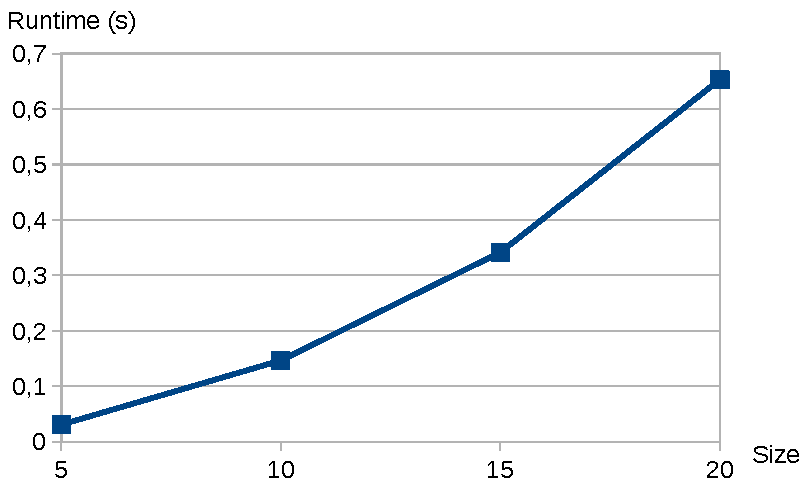
\includegraphics[width=.45\textwidth]{figures/performance/star2wheel}
	\caption{The arithmetic average of the execution times of several runs of \emph{Star2Wheel} transformations with example input graphs whose sizes range from 5 to 20 on the BNCE transformer}
	\label{fig:performance-star2wheel}
\end{figure}

Figure \ref{fig:performance-star2wheel} displays the result of the performance evaluation for the transformation \emph{Star2Wheel}. For this transformation, we cannot discriminate between star graphs with a certain size $n$ that generate a deep or a shallow parsing tree, because there exists only one such star graph with size $n$ (up to isomorphism). Furthermore, as stated in Section \ref{sec:eval-usability}, we could not model this transformation in standard TGG. Thus, the only line in Figure \ref{fig:performance-star2wheel} refers to the BNCE implementation and evinces the already expected polynomial behavior of the algorithm for connected degree-bounded graphs.

\begin{figure}
	\centering
	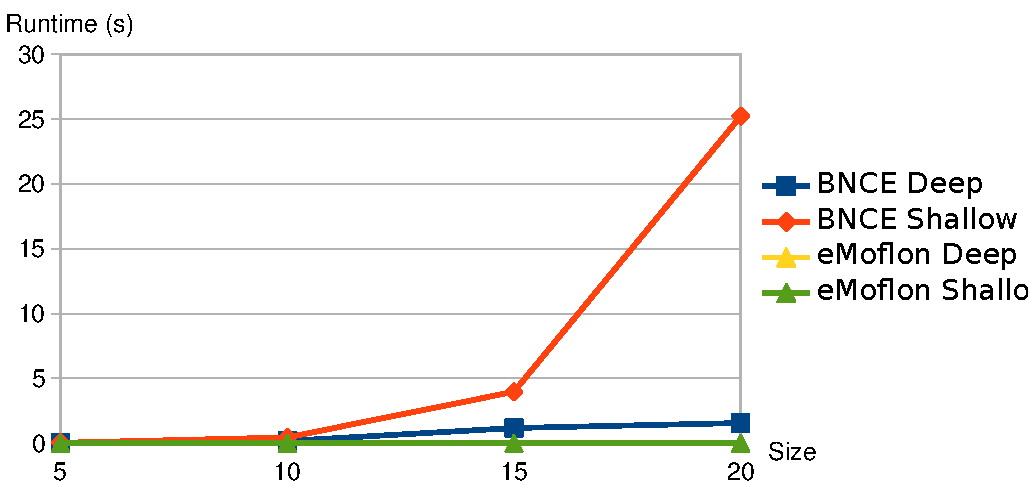
\includegraphics[width=.6\textwidth]{figures/performance/pseudocode2controlflow}
	\caption{The arithmetic average of the execution times of several runs of \emph{Pseudocode2Controlflow} transformations with example input graphs whose sizes range from 5 to 20 and that are discriminated by their parsing trees (\emph{Deep} or \emph{Shallow}) on both implementations (\emph{BNCE} and \emph{eMoflon})}
	\label{fig:performance-pseudocode2controlflow}
\end{figure}

Figure \ref{fig:performance-pseudocode2controlflow} reports on the average runtimes for the \emph{Pseudocode2Controlflow} transformation. For input graphs that generate a deep parsing tree, we perform only slightly worse than eMoflon. However, for the case of shallow parsing trees, the computation time for our implementation grows fast with the inputs' sizes. We think that the good performance of the former case is due to our greedy heuristic that prioritizes the exploration of deeper trees, what enhances the probability of finding the complete parsing tree for these graphs first.

\begin{figure}
	\begin{subfigure}[t]{0.44\textwidth}
		\centering
		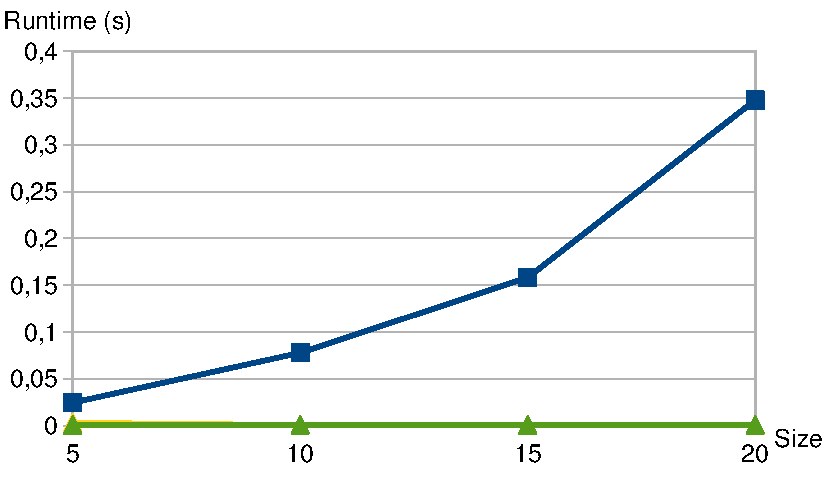
\includegraphics[width=\textwidth]{figures/performance/btree2xbtree-deep}
		\caption{Runtimes only for the class \emph{Deep}}
		\label{fig:performance-btree2xbtree-deep}
	\end{subfigure}
	\begin{subfigure}[t]{0.55\textwidth}
		\centering
		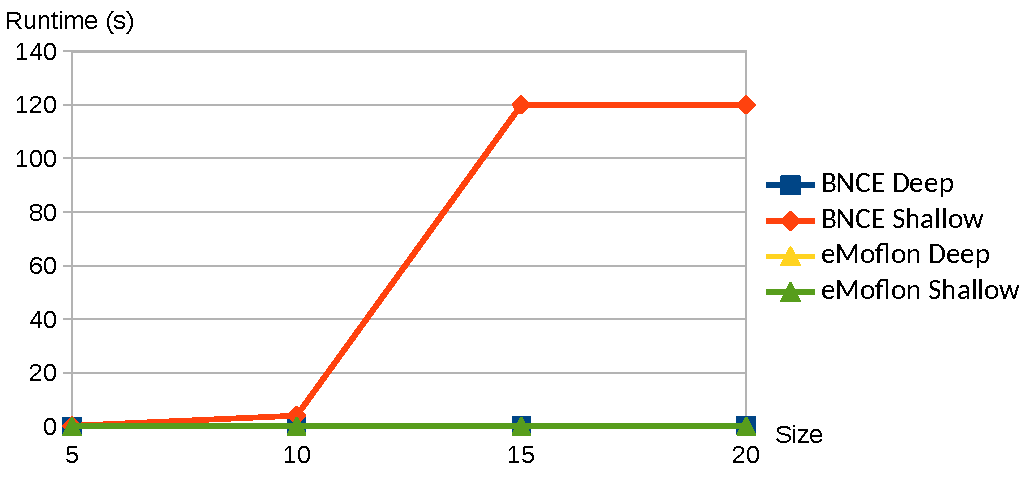
\includegraphics[width=\textwidth]{figures/performance/btree2xbtree}
		\caption{Runtimes for all four classes}
		\label{fig:performance-btree2xbtree}
	\end{subfigure}
	\caption{The arithmetic average of the execution times of several runs of \emph{BTree2XBTree} transformations with example input graphs whose sizes range from 5 to 20 and that are discriminated by their parsing trees (\emph{Deep} or \emph{Shallow}) on both implementations (\emph{BNCE} and \emph{eMoflon})}
\end{figure}

Figure \ref{fig:performance-btree2xbtree-deep} depicts the runtimes for the \emph{BTree2XBTree} transformation for the inputs that generate deep parsing trees on both implementations. Thereby, it is made clear how the BNCE's curve grows faster than the eMoflon's with greater inputs. Indeed, eMoflon's curve seems to be characterized by a polynomial with a much smaller degree than the BNCE's.

Figure \ref{fig:performance-btree2xbtree} depicts the runtimes also for the \emph{BTree2XBTree} case where the two classes of inputs on both implementations are evaluated. This result demonstrates how our implementation performs bad for the class of shallow parsing tree. In particular, the runtime function grows vertiginously for input sizes greater than 10. Notice that, the runtimes are limited by 120s, as we set this timeout in our configuration. Therefore, it is fair to assume, that the real runtime for this class is even worse.

\begin{figure}
	\centering
	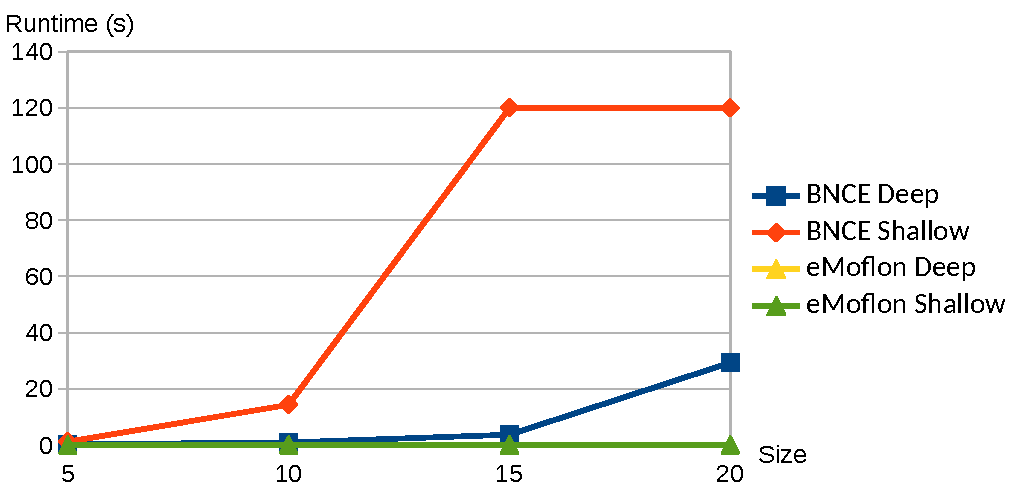
\includegraphics[width=.6\textwidth]{figures/performance/statemachine2petrinet}
	\caption{The arithmetic average of the execution times of several runs of \emph{Statemachine2Petrinet} transformations with example input graphs whose sizes range from 5 to 20 and that are discriminated by their parsing trees (\emph{Deep} or \emph{Shallow}) on both implementations (\emph{BNCE} and \emph{eMoflon})}
	\label{fig:performance-statemachine2petrinet}
\end{figure}

Figure \ref{fig:performance-statemachine2petrinet} reports on the runtime evaluation of the \emph{Statemachine2Petrinet} transformation for the two classes of inputs on both evaluated implementations and shows again the disadvantage of our BNCE TGG implementation against eMoflon, specially for the shallow parsing tree case. The performance evaluation of our implementation at this case resembles very strongly the evaluation of a CYK graph grammar parser presented by \citep[p. 83-90]{hoffmann2017generating}.

\begin{figure}
	\centering
	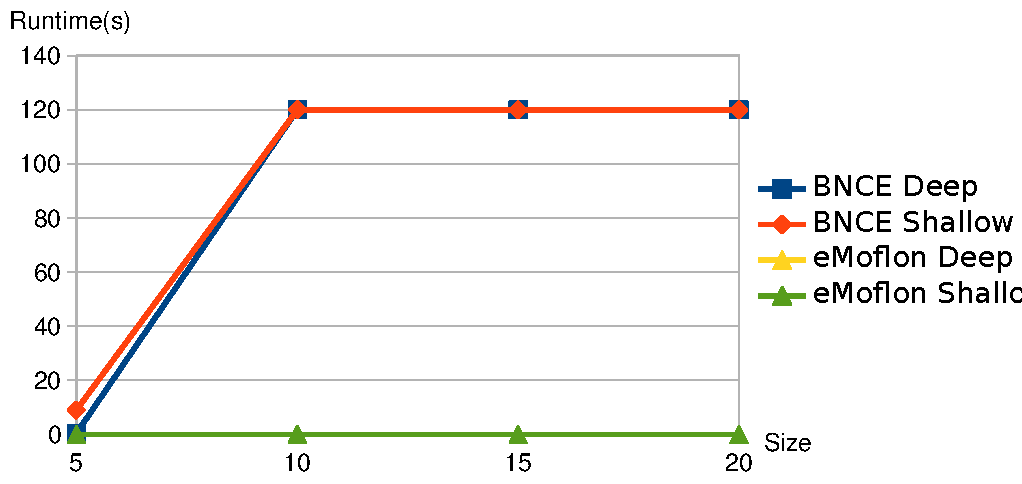
\includegraphics[width=.6\textwidth]{figures/performance/class2database}
	\caption{The arithmetic average of the execution times of several runs of \emph{Class2Database} transformations with example input graphs whose sizes range from 5 to 20 and that are discriminated by their parsing trees (\emph{Deep} or \emph{Shallow}) on both implementations (\emph{BNCE} and \emph{eMoflon})}
	\label{fig:performance-class2database}
\end{figure}

Lastly, Figure \ref{fig:performance-class2database} presents the worst performance result of our approach, which is the one for the \emph{Class2Database} transformation. For this case, our solution is impracticable even for inputs of size 10 that generate deep parsing trees, whereas eMoflon presents a very good performance for both classes of inputs. We cannot explain this phenomenon exactly, but the following reasoning about the time complexity of the BNCE TGG transformer may shed a light on it.

The worst-case time complexity of the BNCE TGG transformer is polynomial in the size of the input graphs, for degree-bounded connected graphs, but the degree of this polynomial is unknown, as far as our knowledge goes. For the general case, the problem of transforming an input graph with a BNCE TGG is NP-complete. This diagnose is valid because the BNCE TGG transformer's complexity is dominated by the parser's, which is proven to be polynomial for the connected case with bounded degree and NP-complete for the general case, according to Rozenberg et al. \cite[p. 160]{rozenberg1986boundary}. That the total algorithm's complexity is dominated by the parser is easy to see in Figure \ref{fig:implementation-scheme}, for the step \emph{Ecore to Graph}'s computational effort is linear on the size of the input model and the step \emph{NP Normalization} is dependent only on the grammar's size (what is considered to be constant) and, finally, the step \emph{Production}'s effort is linear on the length of the derivation, which in turn is also linear on the size of the input graph.

In more details, the parser's complexity can be roughly described as the multiplication of two factors: the number of loop iterations executed until the desired final zone vertex is found (Lines 4 to 15 in Algorithm \ref{alg:parsepac}) and the cost of operations necessary to find the derivations for a handle (Lines 5 to 14 in Algorithm \ref{alg:parsepac}). The latter is clearly a function on the size of the grammar, that is defined through the number of rules and the sizes of right-hand sides and are considered to be constant. The former corresponds to the size of the $bup$ set, which, in turn, is polynomial in the size of the source graph, for a degree-bounded connected graph \cite[p. 161]{rozenberg1986boundary}, but not polynomial in the general case (unless $P=NP$).

Concerning worst-case space complexity, the BNCE parsing problem is NL for degree-bound connected graphs \cite{kim2001efficient} and PSPACE-complete for the general case \cite{rozenberg1986boundary}, what means that the parsing algorithm runs in non-deterministic log-space for the former case and in polynomial-space for the latter. It is also clear that the space complexity of the BNCE transformer is dominated by the parser. In practice, our implementation consumes more space than the necessary, since we keep in memory copies of input's subgraphs that correspond to parsing trees found through the exploration of the parsing tree space. In this sense, our memory consumption could be lessened.

In summary, our approach's performance is not sufficiently good for the general case and is clearly outperformed by eMoflon, specially when the parser generates a shallow parsing tree for the input. One could argue that our transformer is still applicable for the case of deep parsing trees, but, in the practice, this would imply a too strong restriction. As a solution for this issue, we believe that a top-down parser could enhance our transformer's performance considerably, in spite of the probably necessary backtracking. Indeed, eMoflon applies a top-down parser that does not need to backtrack, what guarantees its good performance.